%{{{ Formatierung

\documentclass[a4paper,10pt]{article}

\usepackage{physics_notetaking}

%%% dark red
%\definecolor{bg}{RGB}{60,47,47}
%\definecolor{fg}{RGB}{255,244,230}
%%% space grey
%\definecolor{bg}{RGB}{46,52,64}
%\definecolor{fg}{RGB}{216,222,233}
%%% purple
%\definecolor{bg}{RGB}{69,0,128}
%\definecolor{fg}{RGB}{237,237,222}
%\pagecolor{bg}
%\color{fg}

\newcommand{\td}{\,\text{d}}
\newcommand{\RN}[1]{\uppercase\expandafter{\romannumeral#1}}
\newcommand{\zz}{\mathrm{Z\kern-.3em\raise-0.5ex\hbox{Z} }}
\newcommand{\id}{1\kern-.258em1}

\newcommand\inlineeqno{\stepcounter{equation}\ {(\theequation)}}
\newcommand\inlineeqnoa{(\theequation.\text{a})}
\newcommand\inlineeqnob{(\theequation.\text{b})}
\newcommand\inlineeqnoc{(\theequation.\text{c})}

\newcommand\inlineeqnowo{\stepcounter{equation}\ {(\theequation)}}
\newcommand\inlineeqnowoa{\theequation.\text{a}}
\newcommand\inlineeqnowob{\theequation.\text{b}}
\newcommand\inlineeqnowoc{\theequation.\text{c}}

\renewcommand{\refname}{Source}
\renewcommand{\sfdefault}{phv}
%\renewcommand*\contentsname{Contents}

\newenvironment{Figure}
        {\par\medskip\noindent\minipage{\linewidth}}
        {\endminipage\par\medskip}

\pagestyle{fancy}

\sloppy

\numberwithin{equation}{section}

%}}}

\begin{document}

%{{{ Titelseite

\begin{titlepage}
        \title{5 (1.\ Halbtag) $|$ Operationsverstärker}
        \author[1]{Angelo Brade\thanks{s72abrad@uni-bonn.de}}
        \author[1]{Jonas Wortmann\thanks{s02jwort@uni-bonn.de}}
        \affil[1]{Rheinische Friedrich--Wilhelms--Universität Bonn}
        \date{\today}
\end{titlepage}

\maketitle
\pagenumbering{gobble}

%}}}

\newpage

%{{{ Inhaltsverzeichnis

\fancyhead[R]{\leftmark}
%\fancyhead[R]{\leftmark\\\rightmark}
\fancyhead[L]{\thepage}
\fancyfoot[C]{}

\tableofcontents

%}}}

\clearpage

%{{{

\pagenumbering{arabic}

\begin{multicols}{2}

        \section{Introduction}
        This experiment deals with the opamp and its funcitonality in different circuits.
        The opamp can be used as a non--inverting or inverting amplifier, adder, differential amplifier, current source, monoflop, to logarithmize or exponentiate and to differentiate or integrate a signal.
        It is also possible to build a \textsc{Schmitt}--trigger or an astable multivibrator.
        In this experiment the opamp will serve as a non--inverting amplifier, adder, current source, integrator and differential amplifier.

        \section{Theory}
        \begin{Figure}
                \centering
                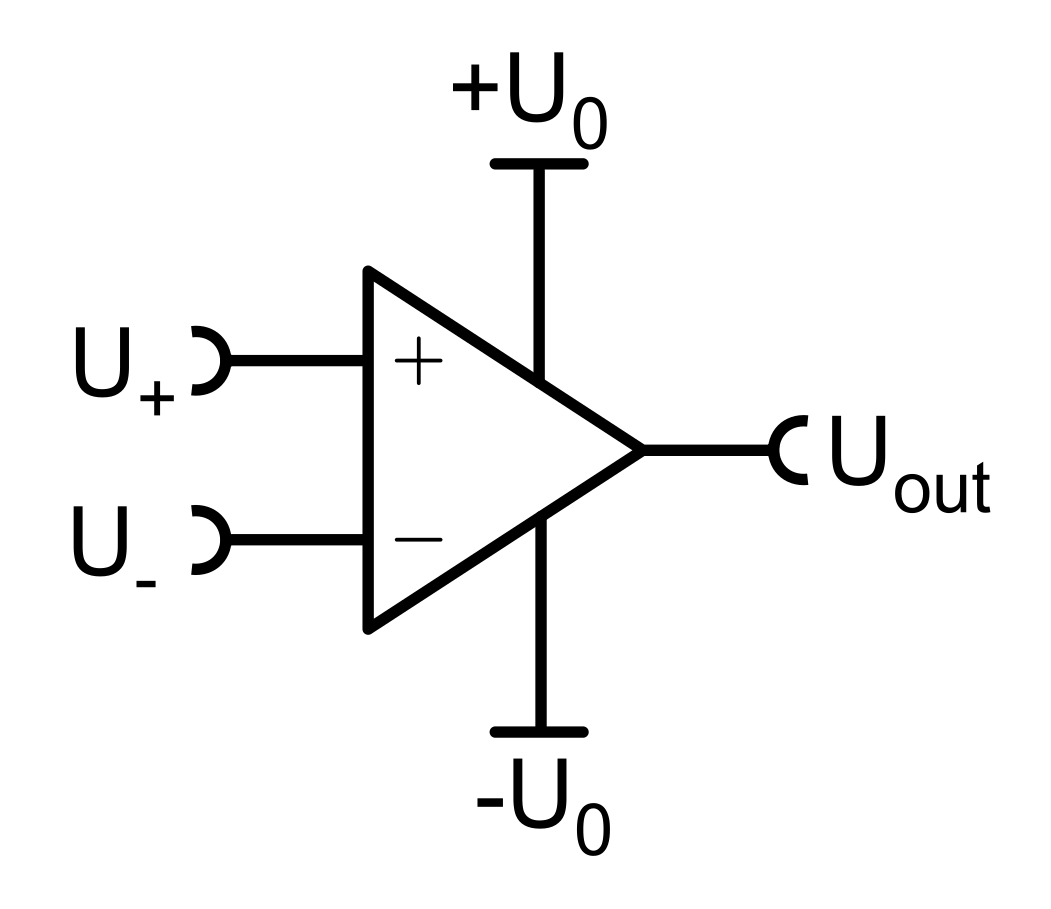
\includegraphics[width=0.5\textwidth]{opamp.png}
                \captionof{figure}{Schematic of an opamp; Abb.\ 5/6.1\cite{Praktikumsanleitung}}
        \end{Figure}
        \noindent The most important properties of opamps are
        \begin{enumerate}[label=--]
                \item With stable negative feedback, the opamp regulates the output voltage such that $U_+=U_-$.
                \item There is close to no input current $I_+=I_-\approx 0$.
        \end{enumerate}
        Important features of real opamps to keep in mind
        \begin{enumerate}[label=--]
                \item The maximum output voltage can't be higher than the maximum supply voltage.
                \item Due to internal constrains, the opamp has a finit slew rate, meaning that it can't change a signal at infinite speed.
                \item The open--loop gain decreases with rising frequency.
                        The bandwidth is the cutoff frequency at which $\nu =\tfrac{1}{\,\sqrt[]{2}}$.
                \item For $U_+=U_-=0$ one would assume that $U_\text{out}=0$.
                        In real world opamps this is not the case.
                        The output voltage goes to zero at a certain difference between $U_+$ and $U_-$.
                        This difference is component specific.
                \item The output voltage should not change if both input voltages increae at the same rate.
                        This is not the case in the real world.
                        The common mode rejection ratio is the ratio between the differential gain and common mode gain.
        \end{enumerate}
        The opamp can be utilised as a non--inverting amplifier with an ideal open--loop gain of infinity.
        Here $U_-=k\cdot U_\text{out}$ and $U_+=U_\text{in}$.
        The gain is
        \begin{align} 
                \nu =\dfrac{U_\text{out}}{U_\text{in}}=\dfrac{1}{k}=1+\dfrac{Z_2}{Z_1}
        .\end{align} 
        \begin{Figure}
                \centering
                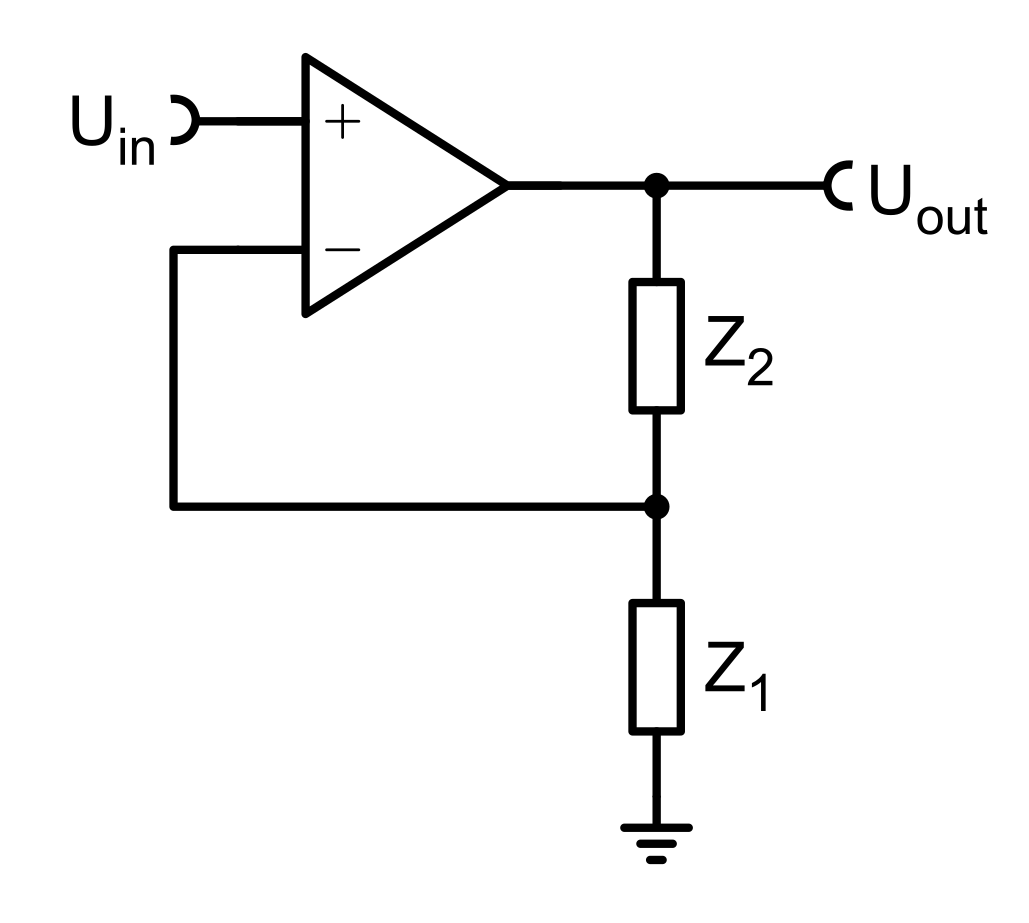
\includegraphics[width=0.6\textwidth]{noninverting_amp.png}
                \captionof{figure}{Non--inverting amplifier; Abb.\ 5/6.4\cite{Praktikumsanleitung}} \label{fig:non--inverting amplifier}
        \end{Figure}
        \noindent The opamp can also be used as an adder.
        As discussed in \hyperref[pre:F]{preliminary task F} the output voltage is an addition of input voltages
        \begin{align} 
                U_\text{out}=c_iU_i\qquad c_i=-\dfrac{R_0}{R_i}
        .\end{align} 
        \begin{Figure}
                \centering
                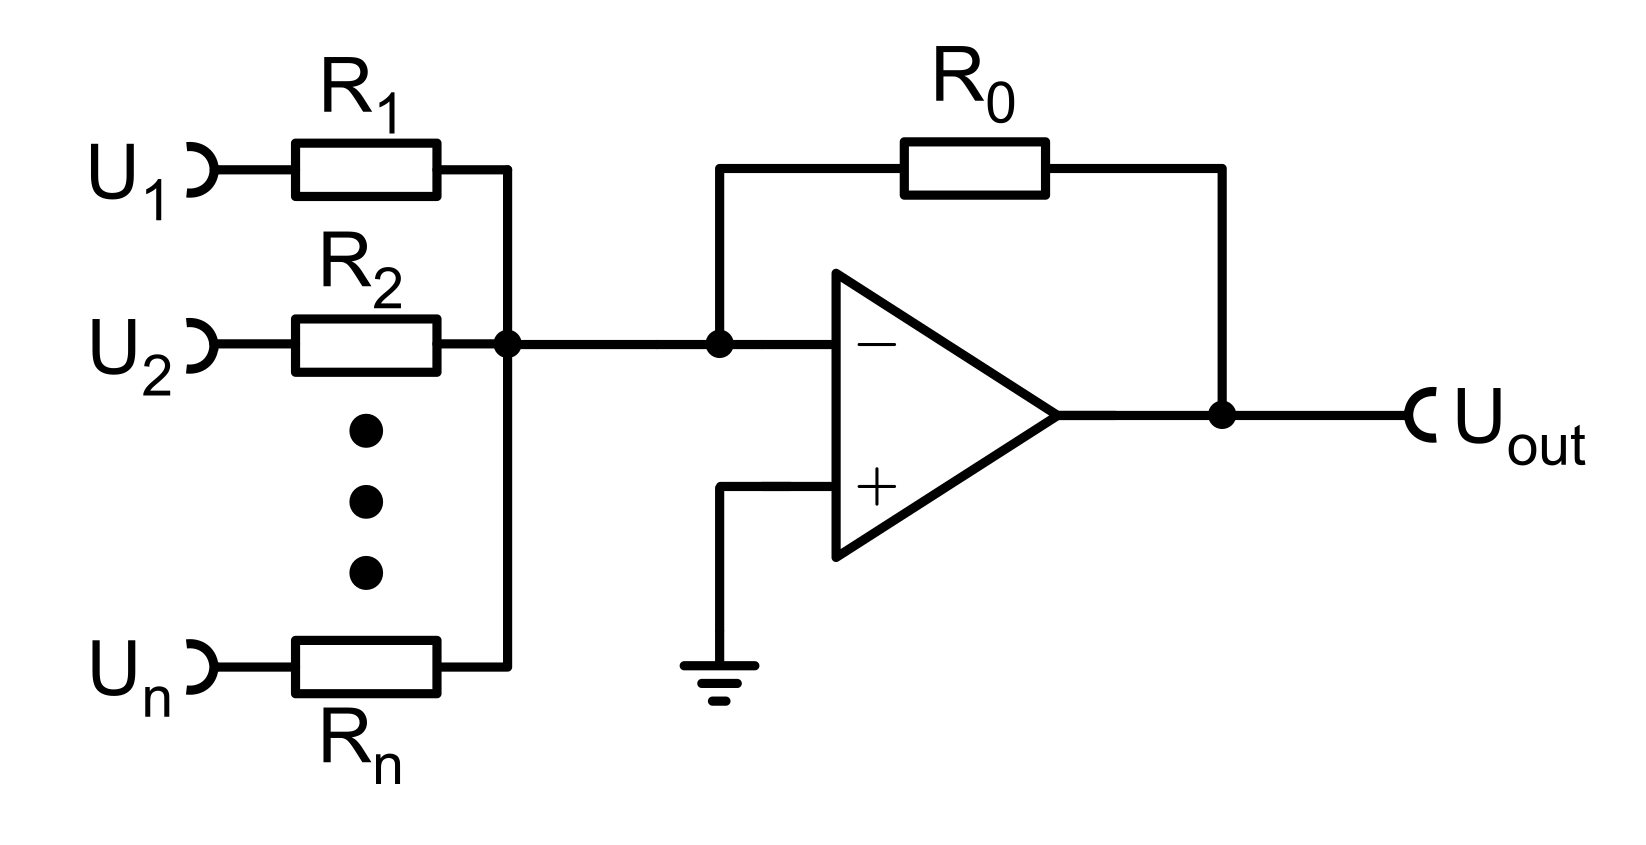
\includegraphics[width=0.6\textwidth]{adder.png}
                \captionof{figure}{Adder; Abb.\ 5/6.6\cite{Praktikumsanleitung}}
        \end{Figure}
        \noindent The opamp can also integrate signals by charging a capacitor to sum up the input signal
        \begin{align} 
                U_\text{out}\left(t\right)=-\dfrac{1}{R_1C}\int_{t_0}^{t}U_\text{in}\left(t'\right)\td t'
        .\end{align} 
        \begin{Figure}
                \centering
                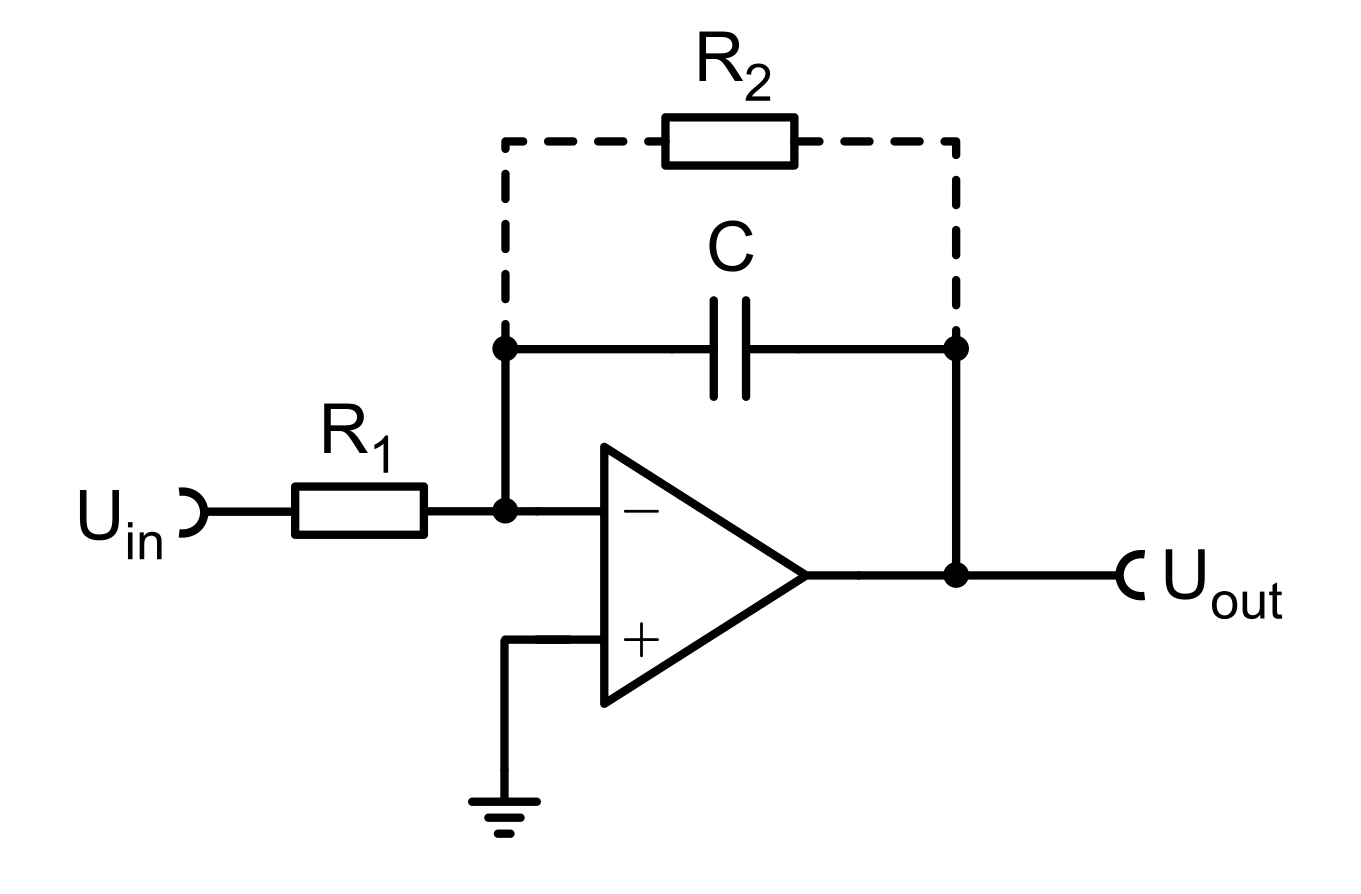
\includegraphics[width=0.6\textwidth]{integrator.png}
                \captionof{figure}{Integrator; Abb.\ 5/6.11\cite{Praktikumsanleitung}}
        \end{Figure}
        \noindent At last the opamp is used in a circuit to function as a differential amplifier.
        As discussed in \hyperref[pre:G]{preliminary task G}, the output voltage is an amplification of the difference of the input voltages
        \begin{align} 
                U_\text{out}=\dfrac{R_2}{R_1}\left(U_2-U_1\right)
        .\end{align} 
        Here $\tfrac{R_2}{R_1}$ is the gain.
        \begin{Figure}
                \centering
                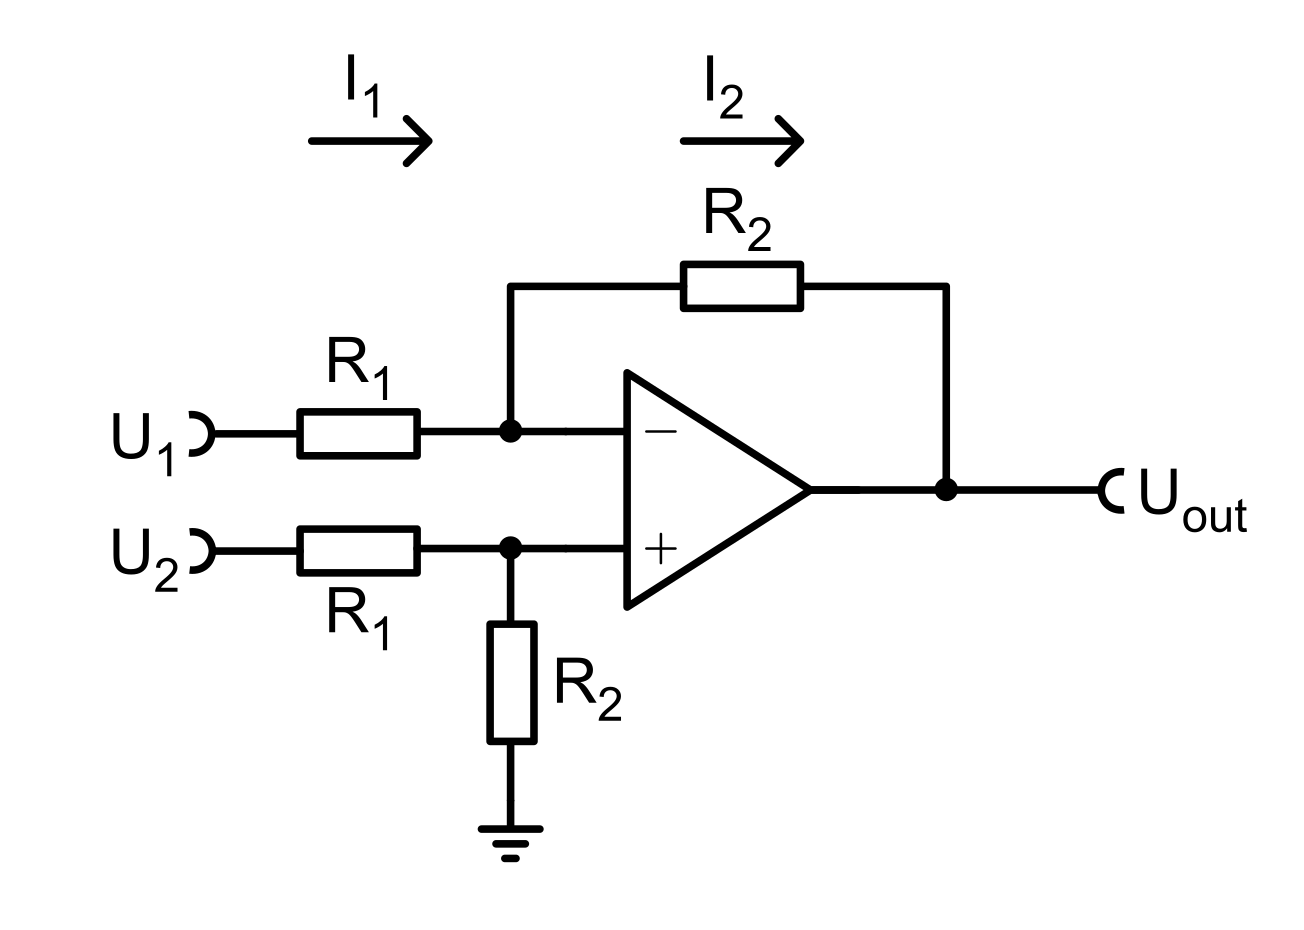
\includegraphics[width=0.6\textwidth]{differential_amp.png}
                \captionof{figure}{Differential amplifier; Abb.\ 5/6.7\cite{Praktikumsanleitung}}
        \end{Figure}
        \noindent When using the opamp as an inverting amplifier, the current flowing through the negative feedback circuit does not depend on $Z_2$ but only on $U_\text{in}$ and $Z_1$.
        Thus one can construct a current source for the resistance $Z_2$ which can be controlled via the input voltage.
        \begin{Figure}
                \centering
                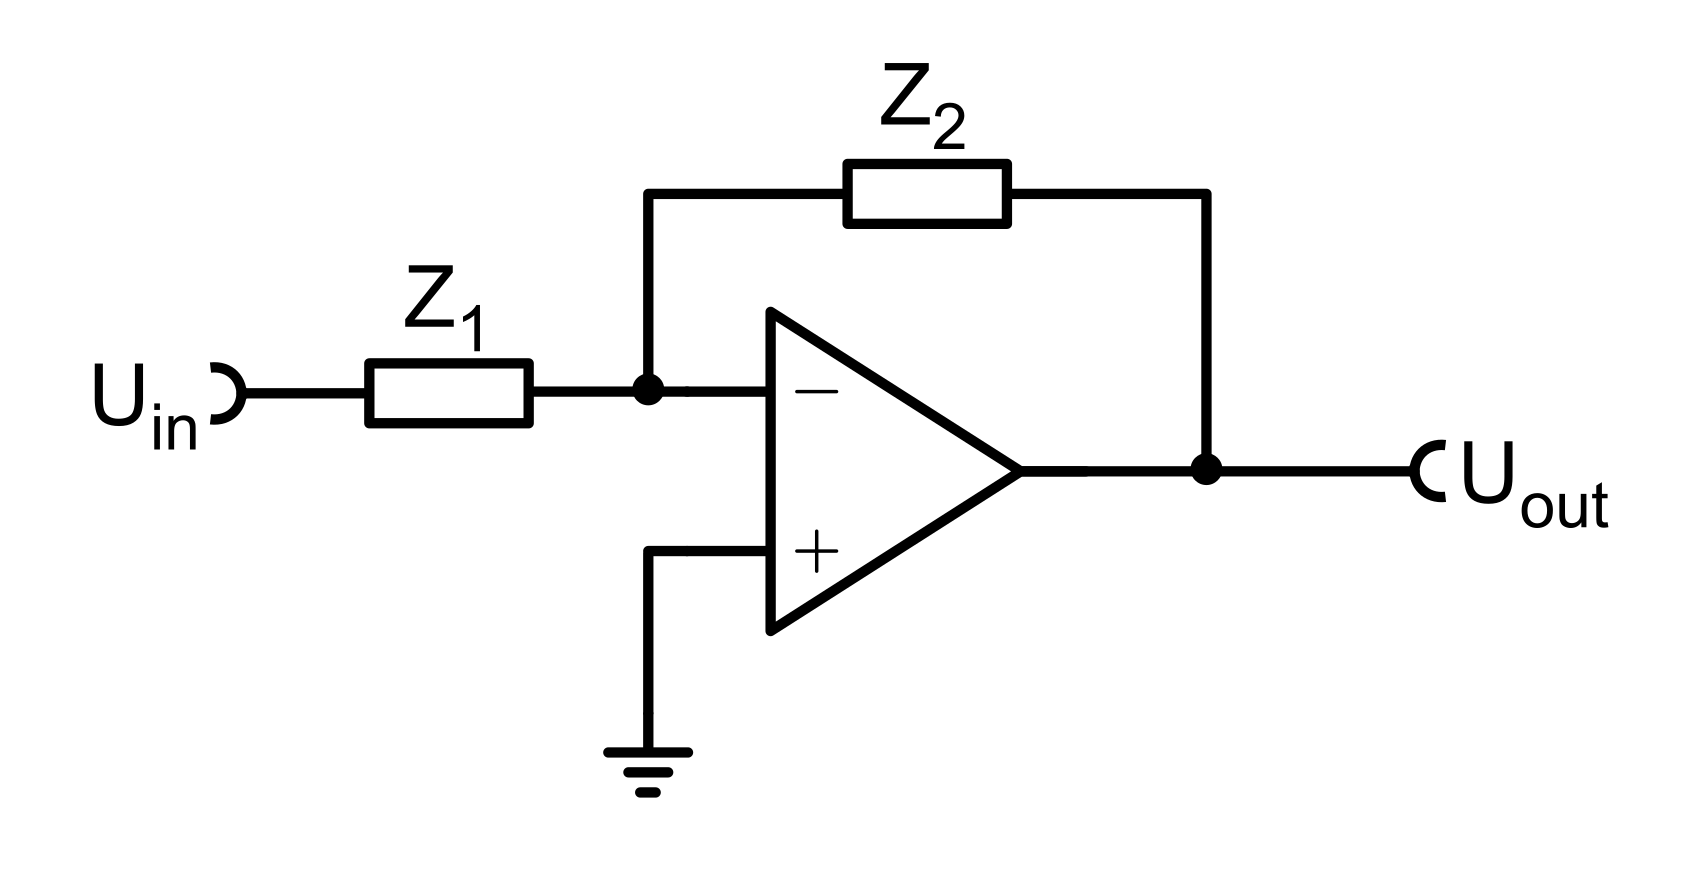
\includegraphics[width=0.6\textwidth]{inverting_amp.png}
                \captionof{figure}{Inverting amplifier; Abb.\ 5/6.5\cite{Praktikumsanleitung}}
        \end{Figure}
        \noindent The astable multivibrator uses the \textsc{Schmitt}--trigger to construct a signal from an ideal wave form, see \hyperref[pre:K]{preliminary task K}.
        \begin{Figure}
                \centering
                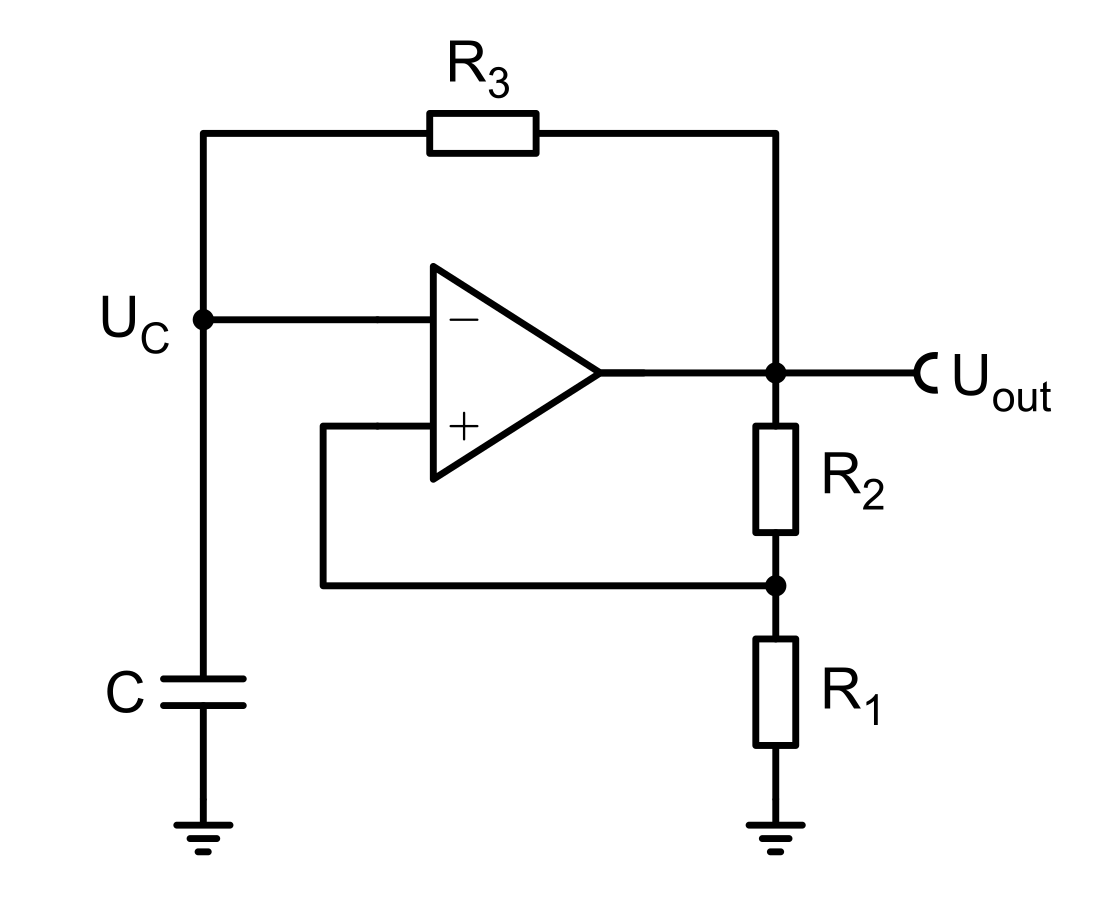
\includegraphics[width=0.6\textwidth]{astable_multivibrator.png}
                \captionof{figure}{Astable multivibrator; Abb.\ 5/6.15\cite{Praktikumsanleitung}}
        \end{Figure}

        \section{Preliminary Tasks}
        \subsection{A}
        The equation hold
        \begin{align} 
                \dfrac{1}{\nu }&=\dfrac{1}{\nu _0}+k&\nu &=\dfrac{1}{\tfrac{1}{\nu _0}+k}
        .\end{align} 
        For $k=0.1$, $\nu _0=10^4$ and $\nu _0=10^5$
        \begin{align} 
                \nu _1&\approx 9.990 & \nu _2&\approx 9.999
        .\end{align} 
        The approximation $\nu =\tfrac{1}{k}$ results in
        \begin{align} 
                \nu _\text{Näh}&=10
        .\end{align} 
        The deviation of $\nu _1$ and $\nu _2$ from $\nu _\text{Näh}$ lie at $0.001\%$ and $0.0001\%$ respectively.

        \subsection{B}
        It hold
        \begin{align} 
                &&&& U_x &= U_\text{in}-kU_\text{out} &&&& \\
                &&\Leftrightarrow && &= U_\text{in}-kv_0U_x &&&&\nonumber \\
                &&\Leftrightarrow && &= \dfrac{U_\text{in}}{1+v_0k}. &&&&
        \end{align} 
        For $k=0.1$, $v_0=10^5$ and $U_\text{in}=\SI{1}{V}$
        \begin{align} 
                U_x\approx \SI{0.0001}{V}
        .\end{align} 

        \subsection{C}
        Let there be a common mode signal with $\Delta U_+=\Delta U_-=+\Delta U_\text{in}$.
        then
        \begin{align} 
                &&&& \Delta U_+ &= \Delta U_E+\Delta U_1 & \Delta U_- &= \Delta U_E+\Delta U_1. &&&& 
        \end{align} 
        from this follows $\Delta U_\text{in}=\Delta U_E+\Delta U_1$.
        The output voltage is
        \begin{align} 
                \Delta U_\text{out}=R_C\cdot \Delta I_C
        .\end{align} 
        At point 1,
        \begin{align}
                I_1=2I_E
        .\end{align} 
        Therefore
        \begin{multline} 
                \Delta U_\text{in} = R_E\cdot \Delta I_E+R_1 \cdot 2\Delta I_E \\= \Delta I_E\left(R_E+2R_1\right)\approx \Delta I_E\cdot 2R_1.
        \end{multline} 
        At the node $U_\text{out}$ applies
        \begin{align} 
                \Delta I_E=\Delta I_C\Rightarrow \Delta U_\text{out}=R_C\cdot \Delta I_E
        .\end{align} 
        The amplification results in
        \begin{align} 
                v_{CM}=\dfrac{\Delta U_\text{out}}{\Delta U_\text{in}}=\dfrac{R_C}{2R_1}
        .\end{align} 
        The common mode suppression is
        \begin{align} 
                10\log \left(\dfrac{R_E}{R_1}\right)=10\log \left(\dfrac{\SI{1}{\kilo\ohm}}{\SI{100}{\kilo\ohm}}\right)=-\SI{20}{dB}
        .\end{align} 

        \subsection{D}
        The frequency dependence of the impedance of a capacitor is
        \begin{align} 
                Z_1 &= \dfrac{1}{\text{i}\omega C}=\dfrac{1}{\text{i}2\pi fC}\\
                |Z_1| &= \left|\dfrac{1}{\text{i}\omega C}\right| = \dfrac{1}{2\pi fC}
        .\end{align} 
        The gain as a function of frequency is
        \begin{align} 
                v\left(f\right)=1+\dfrac{Z_2}{|Z_1|}=1+R2\pi fC
        .\end{align} 
        The limits are
        \begin{align} 
                \lim_{f \rightarrow 0}\left[1+R2\pi fC\right] &= 1 & \lim_{f \rightarrow \infty}\left[1+R2\pi fC\right] &= \infty
        .\end{align} 
        For $|Z_1| = R$ it has to hold that
        \begin{align} 
                \dfrac{1}{2\pi fC}=R\Leftrightarrow f=\dfrac{1}{2\pi RC}
        .\end{align} 
        With concrete values $Z_1=R=\SI{100}{\kilo\ohm}$ and $Z_1=C=\SI{100}{\nano F}$, the frequency is
        \begin{align} 
                f=\dfrac{1}{2\pi RC}\approx \SI{15.92}{Hz}\Rightarrow v\left(f\right)\approx 2
        .\end{align} 
        \begin{Figure}
                \centering
                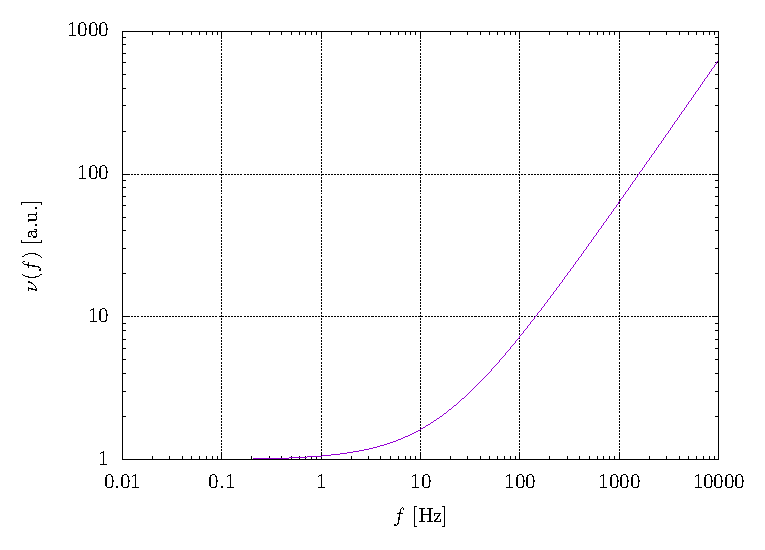
\includegraphics[width=0.7\textwidth]{../plot/preE_crop.pdf}
                \captionof{figure}{Time dependend amplification of a non--invertible amplifier as a \textsc{Bode}--plot}
        \end{Figure}

        \subsection{E}
        Let
        \begin{align} 
                v=\dfrac{U_\text{out}}{U_\text{in}}=-\dfrac{Z_2}{Z_1}
        .\end{align} 
        The minus sign results from the negative feedback.
        Because of the golden rule $U_-=U_+=\SI{0}{V}$, the negative feedback has a different sign compared to the input signal.
        \\\indent The input impedance is very high and the output impedance very low. 

        \subsection{F} \label{pre:F}
        The first \textsc{Kirchhoff}'s law states (\textsc{Einstein} notation)
        \begin{align} 
                &&&& \sum_{i}^{}I_i &= -I_\text{out} &&&& \\
                \Leftrightarrow  &&&& \dfrac{U_i}{R_i} &= -\dfrac{U_\text{out}}{R_0}&&&& \\
                \Leftrightarrow  &&&& -\dfrac{R_0}{R_i}U_i &= U_\text{out} &&&& \\
                \Leftrightarrow  &&&& c_iU_i &= U_\text{out}. &&&& 
        \end{align} 
        
        \subsection{G} \label{pre:G}
        \begin{align} 
                &&&& U_+ &= U_2\dfrac{R_2}{R_1+R_2} &&&& |\text{voltage divider}\\
                &&&& U_- &= U_+ &&&& |\text{golden rule}\\
                &&&& I_1 &= \dfrac{U_1-U_-}{R_1} &&&& |\text{\textsc{Ohm}'s law}\\
                &&&& I_2 &= I_1 &&&& |\text{golden rule}\\
                &&&& I_2 &= \dfrac{U_-U_\text{out}}{R_2} &&&& |\text{\textsc{Ohm}'s law}
        .\end{align}
        The final result $U_\text{out}=\tfrac{R_2}{R_1}\left(U_2-U_1\right)$ can be calculated using the above relations.

        \subsection{H}
        A constant negative input voltage provides a continuous charge to the capacitor, resulting in a steadily rising output voltage.
        One could also argue that for a constant input voltage the integral will increase linearly.

        \subsection{I}
        For an inverting amplifier $\nu =-\tfrac{Z_2}{Z_1}$.
        With $Z_1=R$ and $Z_2=\tfrac{1}{\text{i}\omega C}$ 
        \begin{align} 
                &&&& \nu  &= -\dfrac{1}{\text{i}\omega CR}. &&&& 
        \end{align} 
        The phase relation between the output-- and inputsignal is then
        \begin{align} 
                \tan \Phi  &= \dfrac{\mathfrak{I}\left(\nu \right)}{\mathfrak{R}\left(\nu \right)}=\lim_{\alpha \rightarrow 0}\dfrac{-\tfrac{1}{\omega CR}}{\alpha }=-\infty
        .\end{align} 
        Thus $\Phi =-\tfrac{\pi }{2}$.

        \subsection{J}
        The AD711 opamp has a slew rate of $s=\SI{20}{V.\micro s ^{-1}}$.
        The peak to peak voltage lies at $U_{p p}=\SI{28}{V}$.
        This means that the AD711 needs
        \begin{align} 
                t=\dfrac{U_{p p}}{s}=\SI{1.4}{\micro s}
        \end{align} 
        to get from $\SI{-14}{V}$ to $\SI{+14}{V}$.
        The switching frequency is therefore
        \begin{align} 
                \tfrac{1}{t}=\SI{0.714}{\micro s ^{-1}}
        .\end{align} 
        
        \subsection{K} \label{pre:K}
        \begin{Figure}
                \centering
                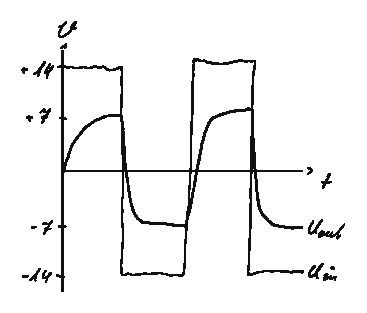
\includegraphics[width=\textwidth]{../plot/preK_crop.pdf}
                \captionof{figure}{Astable multivibrator, voltage curve}
        \end{Figure}
        \noindent The ideal signal is a square--wave with $U_\text{max,min}\pm \SI{14}{V}$.
        Due to the slew rate of the opamp, the signal need time to rise to $\pm \si{7}{V}$.
        The output voltage can be modeled with an exponential function.

        \newpage
        \section{Analysis}

        \subsection{Non--inverting amplifier}
        The \hyperref[fig:non--inverting amplifier]{non--inverting amplifier} is built with a gain of $\nu =11$ (i.e.\ $R_1=\SI{1}{k\ohm}$ and $R_2=\SI{10}{k\ohm}$).
        A signal of $U_{p p}=\SI{1}{V}$ is applied to the circuit and the gain is observed for different frequencies.
        \begin{Figure}
                \centering
                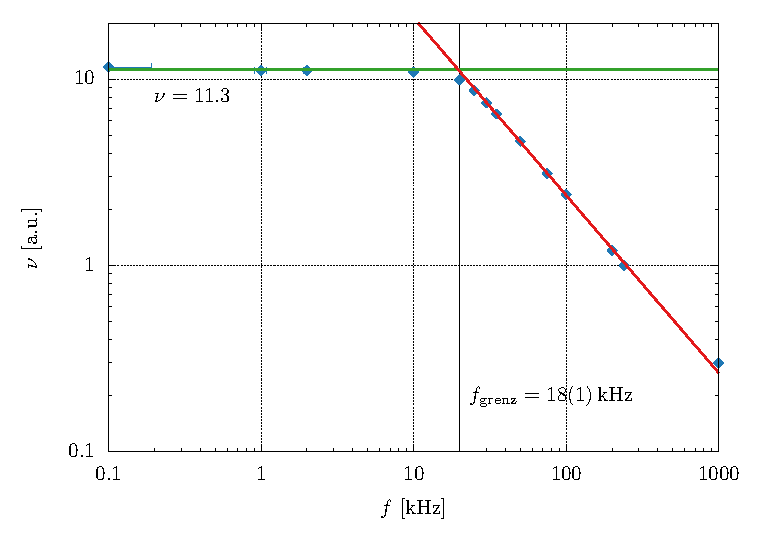
\includegraphics[width=0.6\textwidth]{../plot/5_1_2_crop.pdf}
                \captionof{figure}{\textsc{Bode}--plot of a non--inverting amplifier with $\nu =11$}
        \end{Figure}
\end{multicols}

\clearpage
\listoffigures
\listoftables
\bibliographystyle{plain}
\bibliography{refs}

%}}}

\end{document}
